%!TEX root = ../thesis.tex
% User scenario using the DemoDraw system

\begin{figure*}[!th]
  \centering
  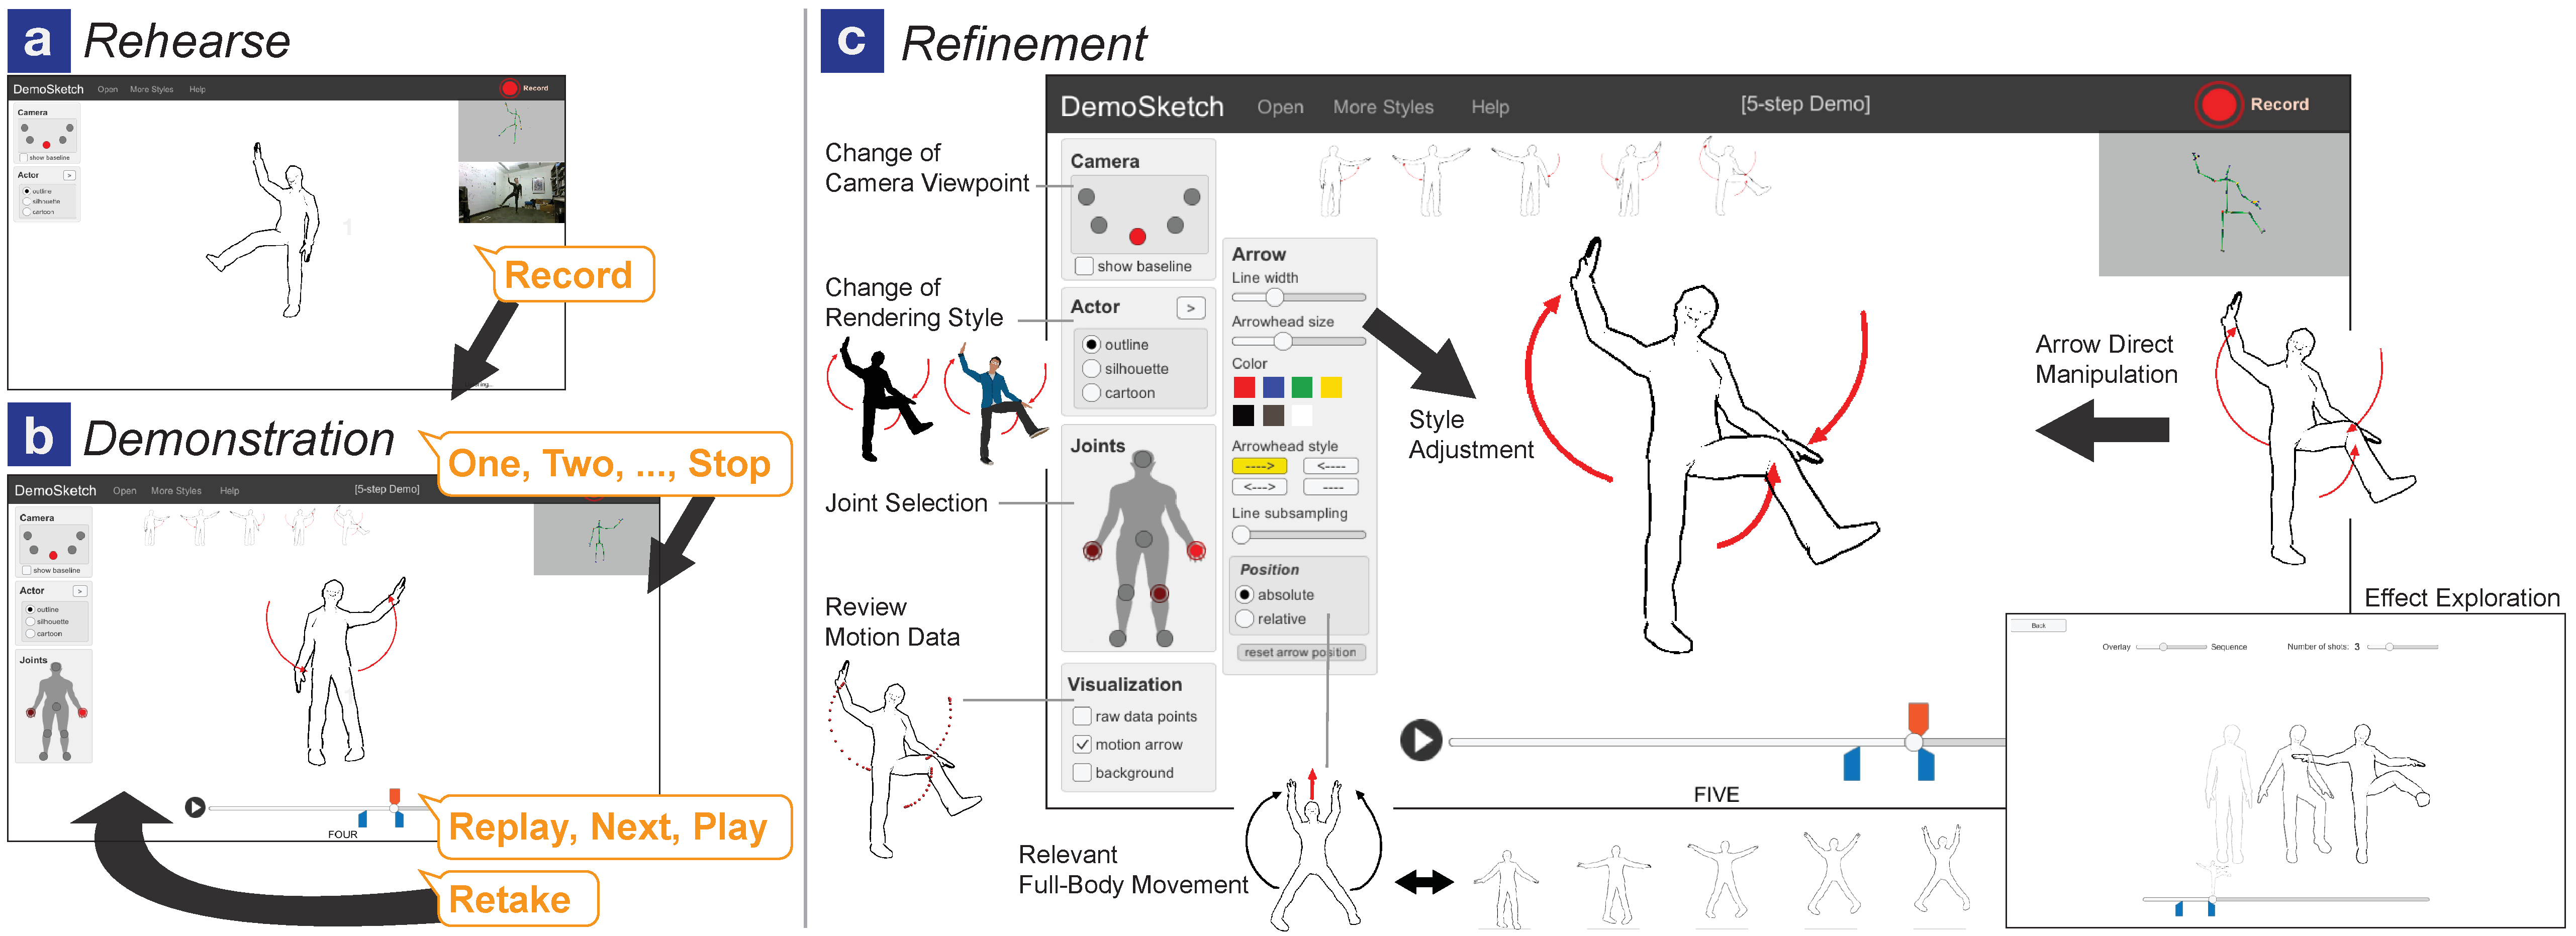
\includegraphics[width=0.8\textwidth]{\demodraw/fig/ui/ui}
  \caption{\systemname{} authoring UI: Using the \phaseI{}, an author sees an avatar following her real-time movement (a). During recording (initiated by voice command ``Start''), real-time feedback shows the speech labels (b). Once a recording is completed by voice command ``Stop'', the motion visualization and a timeline are immediately available (c) for the author to review, and a step-by-step overview will be generated.}
  \dan{I changed figure start command to Start to match the video.}
  \label{fig:DemoDrawUI}
\end{figure*}

\clearpage

\section{Multi-Modal Authoring}
% \dan{Somewhere in this section need to justify need for motion re-taking and/or motion editing based on \textbf{three kinds of possible errors}: 1) user not happy with their own motion performance; 2) user not happy with quality of Kinect capture; 3) user not happy with system's motion segmentation or identified salience.}\bjoern{I'd add 4) based on illustration review, users decides to change performance to increase legibility.}

\systemname{} is designed for non-experts who cannot effectively or efficiently create concise motion illustrations motions using existing tools.
% This is achieved using two modes, the \phaseI{} and the \phaseII{}.
% \dan{The term ``phase'' implies a non-iterative sequential ordering. ``interface'' may not be good either if the UI is actually the same (I thought it was a bit different when they stood back for demonstration, but I guess not). Perhaps ``mode'' is best.)}
% \peggy{I agree and have changed the term in the paper}
To provide an overview of how the system works, we present a scenario in which a motion illustration author, Marie, creates instructions for an 8-step dance tutorial.

In her living room, Marie begins using \systemname{} with the \phaseI{} shown on her television by standing in front of a Kinect. In the center of the display, an avatar follows her movements in real-time (Figure~\ref{fig:DemoDrawUI}a).
 % with a smaller skeleton view and RGB video stream for recognition verification (Figure~\ref{fig:DemoDrawUI}-1b). \bjoern{I think you can get rid of the skeleton and perhaps also RGB video - those are debugging views for you.}
% \dan{just put one label for skeleton and RGB since these aren't a big focus}
This avatar is shown as an ``outline'' figure, but she could always change to different rendering effects like ``silhouette'' or ``cartoon,'' or select a different 3D human model later using our \phaseII{} (Figure~\ref{fig:DemoDrawRefinementUI}a).
% \dan{how does she select these while standing in front of the kinect? If she needs to use the \phaseII{} then let's talk about them there or have her pick them using the \phaseII{} before starting the demonstration.} \bjoern{yeah, i was wondering about this too}


\subsubTitleBold{Recording}
Marie starts recording her physical demonstration with the voice command \iquote{Start.} After a 3-second countdown, \systemname{} captures the position, orientation, and depth distance of her body (using Kinect's simplified 25 body joint model).
%
While demonstrating dance moves, Marie verbally indicates the count of each step with \iquote{one, two, three, and four,} just like she does when teaching a dance. The specific utterance is not constrained, Marie could use words like \iquote{right, left, shake, and clap.} A speech recognition engine captures these labels with timestamps and displays them in the interface (Figure~\ref{fig:DemoDrawUI}b).
Marie finishes recording by saying \iquote{Stop}.

\subsubTitleBold{Reviewing and Re-Recording}
After recording, \systemname{} automatically segments the motion around the speech labels and identifies salient joints. An illustration of the first step of Marie's demonstration is rendered with motion arrows, showing the path of the most salient joints. Figure~\ref{fig:DemoDrawUI}c presents an example illustration that shows how her right hand waves from bottom to the top, and the left on the opposite direction. She also notices three panels emerged: A timeline below shows the start, end, and key frame points used to generate the current illustration, a side panel shows the visualized joints; an step-by-step overview of step snapshots is created and added to a motion sequence list.
%
Marie can navigate to other illustrated steps by either saying \iquote{Next} or \iquote{Back}, or repeating one of the words she said during recording (like \iquote{three}) to skip to that corresponding step. To play an animation showing her continuous motion, she can say \iquote{Play} to play the current step only, or \iquote{Replay} to play the entire motion recording with each step visualization highlighted.

Once Marie reviews the steps, she realizes she should have exaggerated the hand motion in step 4. By saying \iquote{Retake Four,} Marie can re-record a partial sequence of movements including that step (e.g., redoing and saying ``Four'' and ``Five'').
When she ends the re-recording with \iquote{Stop}, the old illustration for that step is replaced with a new one (step four in this example) generated using the new motion recording.
%
% Furthermore, \systemname{} supports hand gestures for certain operations. For each step, \todo{Marie could adjust the start and end time of the motion using her left and right hands respectively.} By saying \iquote{Adjust}, she slowly moves her right hand to the right to extend the end time. She says \iquote{Done} to save the changes. She could always say \iquote{Cancel} to clear any recording or editing operation.
% No undo/redo
%
% TODO!! \dan{It would be so cool to have functionality to add and remove joints using the Kinect only: Marie finds that only her right hand was recognized as salient, but she wants a very subtle movement with her left hand to be shown too. She says \iquote{Add} while moving her left hand and the system adds her left hand's motion to the illustration. She can also say \iquote{Remove} to remove a joint from motion depiction.}

\begin{figure*}[t!]
  \centering
  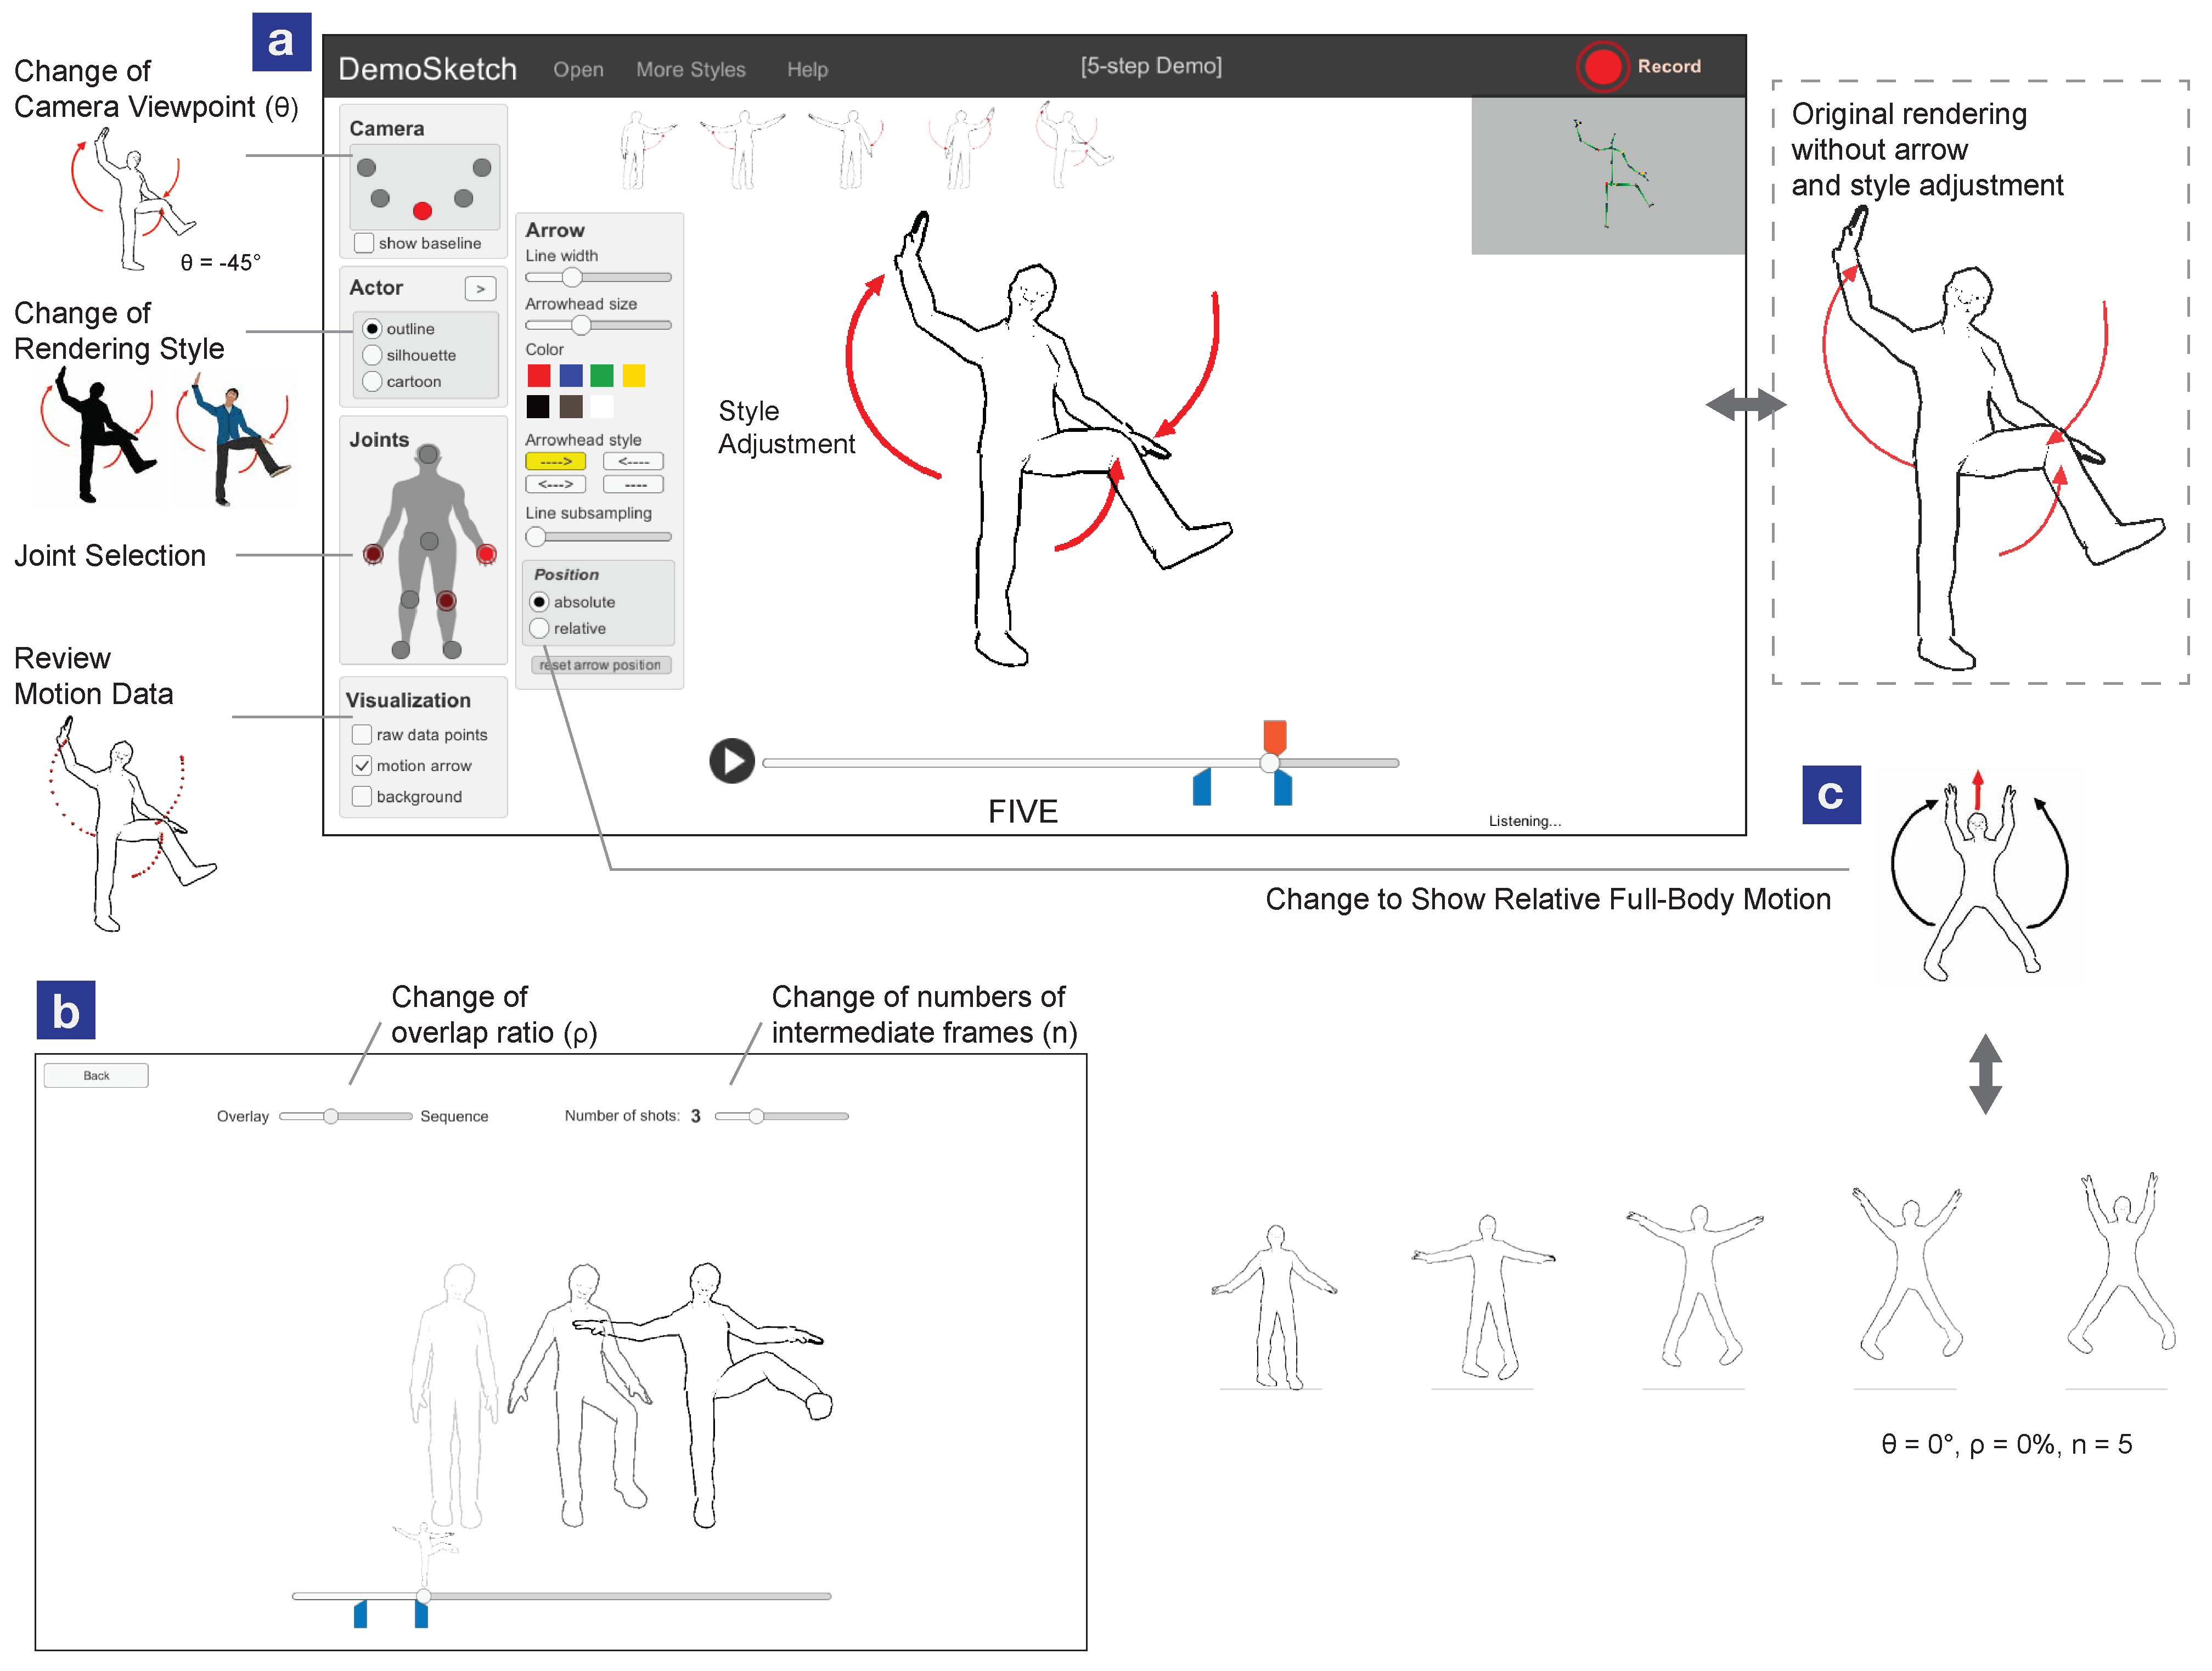
\includegraphics[width=\textwidth]{\demodraw/fig/ui/refinement_ui}
  \caption{Using \systemname{}'s \phaseII{}, the author can refine the visuals (a) and explore more illustration effects (b, c).}
  \label{fig:DemoDrawRefinementUI}
\end{figure*}

\subsubTitleBold{Motion Depiction Adjustments}
Once Marie is satisfied with her demonstration, she walks out of the capture area to her desktop computer. The system automatically switches to the \phaseII{} by revealing post-processing panels in a standard graphical user interface (Figure~\ref{fig:DemoDrawRefinementUI}a).
% \dan{so there are two interfaces!}
Using this interface, Marie can adjust several design parameters:
% \dan{I rewrite these to match parameters in figure 2 and added some as well.}
the arrow appearance can be refined, including line width, arrowhead size, and color;
the arrow offset can be adjusted with direct manipulation dragging; %to avoid overlap with the avatar figure
the camera viewpoint can be adjusted by orbiting the camera to a side or three-quarter view;
the joints used for motion paths can be added or removed using a panel;
% \dan{I put viewpoint in the ``context task'' in prev section, so may need to say something about not all context parameters needs to be adjusted in \phaseII{}. }
and the smoothed motion trajectory can be toggled on and off.
%
She could also select a different key pose and adjust the start and end times of a motion segment by dragging the markers on the timeline.
% \dan{if no relative vs. absolute adjustments, we may want to remove ``reference frame'' from figure 2}
% \peggy{Add something about relative motion here.}
%
In addition, Marie could explore other illustration styles like stroboscopic rendering by selecting numbers of intermediate frames and how they render in one diagram (Figure~\ref{fig:DemoDrawRefinementUI}b).
%
These results can be exported to image files containing the final motion illustrations. %replace vector files - possible but not implemented

% \dan{are there other motion styles? I commented out text that suggested that but I didn't think there were more than these two.}
 % for one or more steps to illustrate the continuous movement in one figure. By choosing ``More Styles'' from the menu, a dialog reveals for her to explore the effects.

% Beyond rendering motion arrows, the user decides the visualize a list of poses to compare with. She selects the option``Sequence'' from the menu and generates a stop motion sequence, with a default of 3 frames (Figure~\ref{fig:DemoDrawUI}A). She adjusts the start and end points of the whole motion via the timeline markers, and changes the number of shots and their distance to overlay the figures together (Figure~\ref{fig:DemoDrawUI}B).

% \dan{I would leave these out because they aren't really about post-processing design parameters:
% She could also reveal the raw, smoothened motion paths to confirm the captured data (Figure~\ref{fig:DemoDrawUI}B).
% To make sure the motion arrow renders the actual motion, she toggles the option ``motion path'' to reveal the original trails;}

% \fixme{\subsubTitleBold{Output}
% Finally, Marie chooses to output the generated illustrations of 8 dance moves to one step-by-step diagram. \systemname{} also provides other output formats, including step-by-step animated clips with the 3D model (where the viewing angles can be adjusted), or video snippets from the Kinect camera view (which only provides the front viewpoint).}
% \dan{not sure we should even talk about output formats other than motion illustrations since they're the only focus of this paper. We can talk about other formats like video and even MixT in future work or discussion. If you agree, then this whole ``output section'' can be reduced to a final sentence of the previous paragraph.  }
